\documentclass{article}
    % General document formatting
    \usepackage[margin=0.7in]{geometry}
    \usepackage[utf8]{inputenc}
    \usepackage{tabularray}
    \usepackage[fontsize=12pt]{fontsize}
    \usepackage[parfill]{parskip}
    \usepackage{hyperref}
    \usepackage[final]{listings}
    \usepackage[T1]{fontenc}
    \usepackage{graphicx}
    \usepackage{float}

\hypersetup{
    colorlinks=true,
    linkcolor=blue,
    filecolor=magenta,
    urlcolor=cyan,
}

\setcounter{secnumdepth}{0}
\setcounter{tocdepth}{2}

\title{%
    \bf{Cybersecurity Autumn 2023} \\
    \large Exercises Compendium
}
\author{Magnus Christian Larsen}

\begin{document}

\lstset{
    numbers=left,
    frame=line,
    breaklines=true
}


\maketitle
\vspace*{\fill}
\begin{center}
    \bf{%
        GitHub Username: Autowinto\\
        Student Mail: magla21@student.sdu.dk\\
        Project: https://github.com/Autowinto/JHotDraw\\
        Date: mm/dd/yyyy}
\end{center}
\newpage
\tableofcontents
\newpage
\section{Info}
Questions marked in bold are the important questions for report.\\
Currently in doubt about format of final report. Layout will change.
% \section{Exercise 01: Setting Up the Lab}
VMs installed\\
Networks Set Up
\section*{Exercise 02: Starting the Journey}
\subsection*{Thinking About Threats}
\textbf{Answers based on the following relevant articles:}\\
\begin{itemize}
    \item \href{https://msrc.microsoft.com/blog/2023/07/microsoft-mitigates-china-based-threat-actor-storm-0558-targeting-of-customer-email/}{Microsoft mitigates China-based threat actor Storm-0558 targeting of customer email}
    \item \href{https://blogs.microsoft.com/on-the-issues/2023/07/11/mitigation-china-based-threat-actor/}{Mitigation for China-based threat actor activity}
    \item \href{https://msrc.microsoft.com/blog/2023/09/results-of-major-technical-investigations-for-storm-0558-key-acquisition/}{Results of Major Technical Investigations for Storm-0558 Key Acquisition}
\end{itemize}


\subsubsection*{How did they separate access and infrastructure according to data relevance and impact?}
They perform background checks, have dedicated identifiable accounts, secure access workstations and MFA using hardware token devices. They prevent the use of email and other communication tools which can compromise machines with malware or keylogs. They use Just in Time and Just Enough Access policies. They added the helper APIs, but failed to update relevant endpoint validation. Developers in other teams assumed that this validation was always performed and thus the disconnect happened.

\subsubsection*{How do roles and personnel fit into this, and which role could policies and training play?}
Lack of evidence because of log retention policies. Because of a disconnect between team roles and personnel, validation was not performed.

\subsection*{Pentesting Intro}
\subsubsection*{Which advantages for penetration testing would you see in the different approaches? What is the best option?}

\begin{itemize}
    \item NAT
    \item NAT Networks
    \item Bridged Networking
    \item Host Only
\end{itemize}

\subsubsection*{How does inspecting the ip configuration of a system help you with penetration testing? What is the security relevant aspect?}
It does so by giving you info about all internet adapters, their protocols, their addresses, metrics, etc. etc.

\subsubsection*{How do you get the targeted user to execute our malicious payload?}
Social Engineering, Disguising the file, exploiting vulnerabilities that allow for automatic code execution.

\subsubsection*{Is Metasploitable3 vulnerable to this exploit?}
Testing the vulnerability is simple as connecting to the metasploitable vm and accessing sysinfo, verifying if it's correct.
The vulnerability in this case, is an open nginx 8080 port, allowing us to connect.
Metasploitable3 is very vulnerable to this exploit as it's designed to be so.
It should close unused open ports, regularly update kernel and application versions, shut down unnecessary services and require validation before connection.
It's quite easy to trick someone to download malicious files through torrenting, limewire, linkin-park-in-the-end.exe etc.

\subsubsection*{What is the practical use of this exercise? And why is the payload working in the way it is? How does this exercise relate to remote and reverse shells?}
The practical use of this exercise is to see how easy it is to gain access to a vulnerable systems shell. The payload works how it does because

\subsubsection*{Which folder are you in when you get the meterpreter prompt? And whatis the system-information?}
I am in the folder that the payload.efi was run at

\subsubsection*{As user and the owner of this system -- how would you mitigate this attack?}
By not chmodding and running payloads which I don't know what are smh.

\subsubsection*{How does knowing usernames help an attacker/penentration tester?
}
It's a significant advantage as it allows you to brute-force passwords much faster and ensuring that you are actually on a user with specific permissions.

\subsubsection*{Now that you have access to the Metasploitable machine what else can wedo? Get the list of users on this server, using a shell prompt by typing"shell" into the Meterpreter shell.}
TODO

\subsubsection*{How does knowing usernames help an attacker/penentration tester?}
It's a significant advantage as it allows you to brute-force passwords much faster and ensuring that you are actually on a user with specific permissions.

\subsubsection*{Using the meterpreter shell, check the output of the "arp" command. What do you find? Why could this information be relevant?
}
It displays internet-to-adapter address tables and when you're connected to a target machine, it shows the tables for that machine, which is very useful information when trying to penetrate.

\subsubsection*{Now lets be on the other side of the fence and investigate suspicious connections to our metasploitable server. Which command can you use to see network status and connections? Is there an anomaly or suspicious connection to our server? What makes it suspicious?}
Unexpected source ip addresses, data transfers when you aren't expecting any, HTTP traffic on an unexpected port etc.
\section*{Exercise 03: General Assessment}

\subsection*{Finding information with whois}
\lstinputlisting[caption={Output of whois for sdu.dk}]{Outputs/E03/whois.txt}
\subsubsection*{What do you learn about SDU's network? In the protocol, note the IP range.}
We learn a whole lot about the network such as the date registered, the expiration date, address of registrant and hostnames.

\lstinputlisting[caption={Output of whois for the ip of sdu.dk}]{Outputs/E03/whoisip.txt}
The IP range is 20.33.0.0 - 20.128.255.255

\subsubsection*{What is the whois information for nextcloud.sdu.dk? What do you observe in comparison to the whois-information you gathered for www.sdu.dk}
\lstinputlisting[caption={Output of whois for nextcloud.sdu.dk}]{Outputs/E03/whoisncip.txt}

The IP range is 130.225.128.0 - 130.225.159.255 for one.

In addition, the output is much more detailed without having to query the ip address instead of the website name.

\subsection*{Question: nmap}
\subsubsection*{Nmap scans can be set up to evade firewalls. Which tags would you use for sending packets with specified ip options?}
To do that you would use --ip-options with one of several options such as "R" to set a record route.
\subsubsection*{Nmap scans can be set up to evade firewalls. Which tags would you use for spoofing your MAC address?}
In that case I would use the tag --spoof-mac with either a specific mac address or 0 passed to use a random one.

\subsection*{Comparing the Tools}
\subsubsection*{Compare your results from each of the previous activities in each question (e.g., sparta vs nessus vs openvas). Take notes and discuss overlaps and differences in results, pros and cons, ease of use for each tool.}

GVM, NESSUS, LEGION, METASPLOITABLE VMs

\subsection*{Collecting the Assessment Information}
Find possible vulnerabilities with metasploitable3 (both Windows and Ubuntu).
State tools and resources used and then select 4 vulnerable services for each of the metasploitable VMs for which you document the following:

\textbf{\dag Service, port number and version number, e.g., FTP 21 vxxxx}
TODO

\textbf{\dag Describe or explain at least one vulnerability that you found for that service, i.e., what is the underlying issue and what can be achieved? How severe is that issue? (You do not have to state how to exploit the vulnerability or go into technical details. We will look into this later btw. The intricate technicalities are mostly outside the scope of the course.) But make sure you describe what possible outcomes of the exploit are, what the impact for a real system were and how criticial you would assess the issue due to the effects, i.e., argue for your assessment}\\
TODO

\textbf{\dag For each of the vulnerabilities in the previous point, note the CVE and/or Source of information about the vulnerability for that version. Using metasploit’s info command might help you here, if you want to go to the command line.}\\
TODO

\subsection*{Completing the Assessment}
\textbf{\dag
    Create a final report, extending the collected information with an overall review of the security concerns in both the Metasploitable-3 Windows and Ubuntu systems, e.g., different criticality levels of the services (an overview of how bad the situation is) and which ones to to be prioritized when addressing security issues (a selection of the most relevant issues for prioritisation). For this use a combination of the results from the tools that you used or one of the tools.\\\\
    Note, that you shouldn’t just copy and paste the severity of the tools you use, but read through the CVE you selected and try to determine how critical it is. I.e., what is the possible impact? Is the service inoperable, or is intellectual property at risk?}\\
TODO
\section{Exercise 04: SQL Injection}
\subsection{Preparation}
\subsubsection{Does it mean the MySQL server is protected against cyber attacks?}
It doesn't necessarily mean that the server is protected against attacks. Restricting the version number is one security measure, but it doesn't mean that the entire server is secure from any and all exploits.

\subsubsection{How could that protection look like?}
Protection against cyberattacks could be things like using strong asswords, restricting access to only certain users or groups, using TLS encryption, disabling unnecessary features in the MySQL server, logging access to the server, updating to the latest versions and security patches frequently, setting up a firewall etc.
\subsubsection{And what exactly would it protect against?}
Hiding the version-number protects against exploits that are available for certain versions of the MySQL server, while making use of general best-practices when it comes to security configuration, ensures that the amount of available exploits are minimized.

\subsection{Spying with SQL Injections}
\subsubsection{Please shortly discuss your opinion of this web server's configuration concerning directly listings}
Directory listings should always be disabled for public websites, as it gives potential bad actors access to information about potential vulnerabilities and files that no user would need access to.

\subsubsection{What type of SQLi attack works? Can you explain why?}
Out of the four options presented, the SQL injection attack that will work, is 'OR 1\=1\#. The reason for this, is because the beginning single quote terminates any string, meaning that SQL will now interpret anything after the single quote, as proper SQL statements. After the single quote, the statement OR 1=1, which is of course always a statement and makes the SQL statement always true, giving us the ability to fetch all data in a table for example.

\subsubsection{What is the \# sign for? Can we generally assume it to do the trick?}
A \# symbol denotes the beginning of a comment, which in the context of an SQL injection attack, effectively has the purpose of ignoring any other SQL that might come after our injection, as we don't really care about that and it reduces the risk of some check being run.

\subsubsection{Include four relevant username/password combinations in your report. What is the issue with the passwords in the database and what could be done to secure them?}

Relevant username and password combinations extracted would be:
\\
\begin{center}
  \begin{tblr}{hlines, vlines}
    ben\_kenobi       & thats\_no\_m00n \\
    darth\_vader      & Dark\_syD3      \\
    anakin\_skywalker & but\_master:(   \\
    jarjar\_binks     & mesah\_p@ssw0rd \\
  \end{tblr}
\end{center}
\subsubsection{Which other problem allows you to get into the machine using ssh? How could this be prevented?}
The fact that I can access the SSH server without having setup a valid SSH key is alarming and should be addressed. You shouldn't be able to access an SSH server with a username and password combination only.

\subsection{Elevation of Privilege}
\subsubsection{Which are the individual issues that allowed us to go from a web interface to root access, and how would you address them as a server's operator to prevent them being exploited? Describe the issues you identified and tryto come up with suggestions on how to fix them}

There were several issues. Below I'll list the issues and explain how I would go about fixing these issues.

\begin{itemize}
  \item The directory listing should never be available publicly. In fact, there is very little reason why it should ever be available. Therefore, this should be made unavailable.
  \item Backend is prone to SQL injection attacks. The backend server should validate the incoming requests, especially when raw SQL is involved, so it isn't as prone to SQL injection attacks as what it clearly is.
  \item SSH server accepts plain username and passwords to connect. SSH server should require a valid SSH key to access. Additionally, the SSH server should only be allowed to connect to from specific IP addresses to limit the potential bad actors.
\end{itemize}

\subsubsection{Can SQL Injection expose an otherwise inaccessible database server?}
So long as there is a way to perform input towards an SQL server, it's possible to expose a database to potentially being attacked. It's all a matter of how well protected the backend accessing the database server is.

\subsubsection{How likely do you think an attack scenario as presented here is?}
This specific scenario is extremely unlikely today. For us to have this easy of access to an SSH server with root privileges even, a perfect storm of security vulnerabilities would need to ve available to us. The only reason we have access to all of these vulnerabilities, are because of the metasploitable3 VM, made specifically to be have these vulnerabilities available. In the real world, it wouldn't be so easy.

\subsection{Using our Foot in the Door for Access to Other Services}
\subsubsection{Is sudo necessary? What do we gain by using it?}
Using sudo specifies the command to be run with root privileges, allowing us to view the location of all files containing the payroll name that we are searching for, no matter what folder it's in. We can find files in other users' owned folders as well as folders in root owned directories like this. While not strictly necessary, it does make for a more complete search, and in this case, allows us to find the file we're looking for.
\subsubsection{Are there other ways to search for a file? Which do you know?}
There exist several commands to search for files.

\begin{itemize}
  \item find: The command we used previously.
  \item grep: Used to search for text within files primarily.
  \item ls | grep: ls used together with piping the result to grep allows for searches.
  \item Fuzzy finders: Fuzzy finders allow for searching in both file contents and searching for file names.
\end{itemize}

\subsubsection{Can you find anything interesting?}
Performing the cat command shows us the contents of payroll.php. The file especially contains something interesting, in that the connection details aren't contained in some environment variables or something other. They are fully exposed, allowing us a full backdoor to the mysql database.
\lstinputlisting[caption={The payroll.php file}, firstline=3, lastline=6]{Outputs/E04/payroll.php}
Interesting information that we can obtain from this are the username, password, hostname as well as the database name.
\subsubsection{What's the username, password and database name?}
\begin{itemize}
  \item Hostname: 127.0.0.1 / localhost
  \item Username: root
  \item Password: sploitme
  \item Datbase Name: payroll
\end{itemize}
\subsubsection{What was the problem with the web application?}
The problem with the web application is that it's accepting user input as string concatenation, which makes it very easy to perform SQL injection.
\subsubsection{Which ports and services were the problem associated with?}
We were able to access the directory listing through the exposed port 80 nginx service, which had directory listing enabled.
\subsubsection{How did you exploit the vulnerability?}
The exposed directory listing allowed us to access the payroll.php application and exploit the SQL injectable web application.
\subsubsection{And what were you able to do?}
Through use of said exploit, I was able to gain access to SSH usernames and passwords and be able to gain access to not only the SSH server, but root access, allowing us to see the entire payroll.php file and gain information on how to gain direct database access.
\subsubsection{How would you suggest to fix the problem? (Do some online research aboutSQL injections solutions.)}
Based on my research, the correct way to fix an SQL injection vulnerability, is to separate the SQL from the data itself and "prepare" the data before being used in the query. In the context of the existing payroll.php application, which uses MySQLi to perform its queries, it should make use of the execute\_query() function, which allows you to define a SQL statement and insert the user input as variables. This way, the variables are prepared properly.
\subsubsection{Draft a shortly and crisply, the relevant parts of a policy trying to prevent these issues.}
The policy to prevent these issues will sound as follows:
\\\\
All database queries must be performed using prepared statements of parameters, so as to protect against SQL injections. Additionally, user input should be validated on the frontend, as well as validated and sanitized on the backend. Database connection details should be fetched from some encrypted environment variables or something similar, to not expose these variables to the eyes of potential bad actors. Systems should regularly be updated and patched to avoid some of the most serious vulnerabilities. Finally, staff should undergo periodic training to ensure that these standards are upheld.

\subsection{Fully Explore Local Accounts}
\subsubsection{What are benefits of performing this scan after already having full access?}
The benefits of performing the scan with full access can be, just that. Having full access and potentially discovering new passwords and usernames to crack. By having root access, we already have access to a potential multitude increase in directories that we can scan for vulenerable passwords, which allows the scan to be potentially much more effective.

\subsection{Post-Exploitation}
\subsubsection{Thinking as an attacker, what would your next steps be?}
First, I would seek to gain some sort of persistence, meaning that even if I was discovered and the system restarted, I could still have access to the machine. This would be in the form of some sort of backdoor.
\\\\
Since I already have root access, I don't need to work towards gaining increased access, however, I would install tools which allow me to gain increased information.
\\\\
Having access to one machine on a network, I would try to discover additional machines that I could access, which could potentially gain me access to even more information. I would do all of this while making sure to leave as few logs as possible, so I wasn't discovered.
\subsubsection{As an operator, what would you do to counteract?}
After discovering that an attack is underway, my first
\section*{Exercise 05: Drupal}

\section{Exercise 6: Social Engineering}

\subsection{Defense}
\subsubsection{Which technical tools can be used to defend against social engineering attacks and against which?}
\begin{itemize}
    \item Email filtering software
          \begin{itemize}
              \item \textbf{Functionality: } The software scans incoming emails for potential phishing attempts or malicious contents, resulting in many obvious attempts at malicious activity being filtered.
              \item \textbf{Protects against: } Protects the user against phishing and email scams such as impersonation attempts.
          \end{itemize}
    \item MFA systems
          \begin{itemize}
              \item \textbf{Functionality: } Adds an additional layer of security by forcing the user to input a dynamically generated code as well as their password when signing in.
              \item \textbf{Protects against: } Protects the user against password leaks, insecure passwords etc.
          \end{itemize}
    \item Antivirus software
          \begin{itemize}
              \item \textbf{Functionality: } Scans systems and programs for known malicious code and quarantines files before they can gain access to or change a system.
              \item \textbf{Protects against: } Protects against viruses, malware, spyware and trojans.
          \end{itemize}
    \item User roles and PAM
          \begin{itemize}
              \item \textbf{Functionality: } User roles allow an organization to specify that a user only has access to very specific things in the organization portals and the entire PAM system monitors access to resources and logs attempts at unauthorized access.
              \item \textbf{Protects against: } Helps mitigate damage of social engineering attacks by limiting access to resources if access to a user account is obtained.
          \end{itemize}
\end{itemize}
\subsubsection{Give examples on how you, as IT-experts, can either stop or mitigate Social Engineering.}
Some ways of stopping or mitigating damage from Social Engineering attacks are as follows:
\begin{itemize}
    \item Implementing strong organizational security policies and ensuring that every employee within the organization is trained to follow these policies and procedures.
    \item Controlling access to the physical organization by unauthorized personnel by implementing security badges, key cards, biometric systems etc.
    \item Implementing phishing detection tools and ensuring regular employee phishing tests, allowing them to fail without catastrophic failure ensuing.
\end{itemize}

\subsection{Experiment: Attack and Defend}
The experiment was performed in a small group.

DAN is a quiet reserved loner. He is trusting, good-natured and lenient. He is conscientious, hard-working, well-organized and punctual. He is calm, even-tempered, comfortable and unemotional. He's down to earth, uncreative, conventional and uncurious.
\subsubsection{Attacker's Perspective}
Based off the information provided about DAN, we believe that the proper course of action to socially engineer him would be an email phishing scam, making use of his trusting and well-organized traits by impersonating the danish tax ministry asking him to update his advance statement to ensure correct tax calculations.

Impersonating an authority figure will let us make use of his calm, unemotional and curious nature as well, as these traits make him unlikely to seek out a second opinion, especially considering tax season beginning around november.
\subsubsection{Defender's Perspective}
The course designed to train DAN on how to avoid being socially engineered needs to cater specifically to his weaknesses. Therefore, the curriculum is as follows:
\begin{itemize}
    \item How to efficiently make use of firewalls, anti-phishing tools and spam filters.
    \item Instilling several rules of thumb in DAN and his way of navigating the workspace:
          \begin{itemize}
              \item Official government communication will never include asking for personal information or direct links to signup pages.
              \item Make use of multi-factor-authentication wherever available.
              \item Involve coworkers or supervisors whenever there is any doubt about the validity of emails.
          \end{itemize}
\end{itemize}
\section{Exercise 07: Brute Forcing Glassfish}
\subsection{Brute Force Attack}
\subsubsection{What does HTTPS actually provide protection for?}
HTTPS is primarily used for ensuring a secure connection between client and server, by implementing TLS and that way protecting from man-in-the-middle attacks.
\subsubsection{Which username/password combination did you find?}
After running the glassfish\_login exploit, the username and password combinations that works is admin and sploit respectively. Of course, the passwords would realistically be much stronger than simply admin and sploit.

\subsubsection{Discuss which security relevant problems are we
    testing with a brute force attack?}
With a brute force attack, we are testing for weak passwords, lack of multi-factor-authentication within the organization, as well as external ip addresses being allowed to sign in.
\subsubsection{Discuss what would be your suggestions to the admin
    in order to address and mitigate this issue?}
One thing that the admin could do is use stronger passwords, this however, doesn't help in the case of a password leak to some database. Therefore, another thing that the admin could do, is introduce multi-factor-authentication when signing in to relevant organization accounts. Additionally, restricting access to specific IP addresses localized where the organization is physically located or allowing access through a specific VPN would go a long way to mitigate this issue.
\subsubsection{How is this attack type related to the internet of things,
    internet routers, and, e.g., virtual machines?}
Brute force attacks relate to the three mentioned platforms in the following ways:
\begin{itemize}
    \item
          \textbf{Internet of Things (IoT)}
          Many IoT devices, such as cameras, smart devices and more, often come with default credentials set, which are usually readily available online. This makes these the perfect target for brute force attacks, as most users don't bother changing the default credentials.
    \item
          \textbf{Internet Routers}
          Internet routers suffer the same issue as IoT devices, as again, routers come with default passwords, which many people don't bother setting. If an intruder is even able to gain physical access to the router, an ethernet cable can be used to open ports without the need of Wi-Fi passwords.
    \item
          \textbf{Virtual Machines}
          Just like with the previous two, many virtual machines come with default passwords, (for example the Kali Linux image that we're using for this course), which allows for potential easy access via brute force attacks. Especially if said virtual machines allow for remote access.
\end{itemize}
\subsubsection{Do you know a way in which HTTPS could make the
    connection more secure against this kind of attack?}
While HTTPS doesn't protect against brute force attacks in and of itself, it does so indirectly, by encrypting all data access, securing login pages and ensuring that the server that the user is communicating with is actually the server that it says it is. This makes it much harder for a malicious entity to perform man-in-the middle attacks and makes it harder for passwords to leak onto potential databases which can be used to brute force.
\section{Exercise 08: Threat Modelling}
\subsection{A Simple Health App Data Flow Diagram}
TODO: Write a more coherent text? Maybe? Maybe not? Do I really care?
\begin{figure}[H]
  \caption{Data Flow Diagram for the Health App}
  \vspace*{1em}
  \begin{center}
    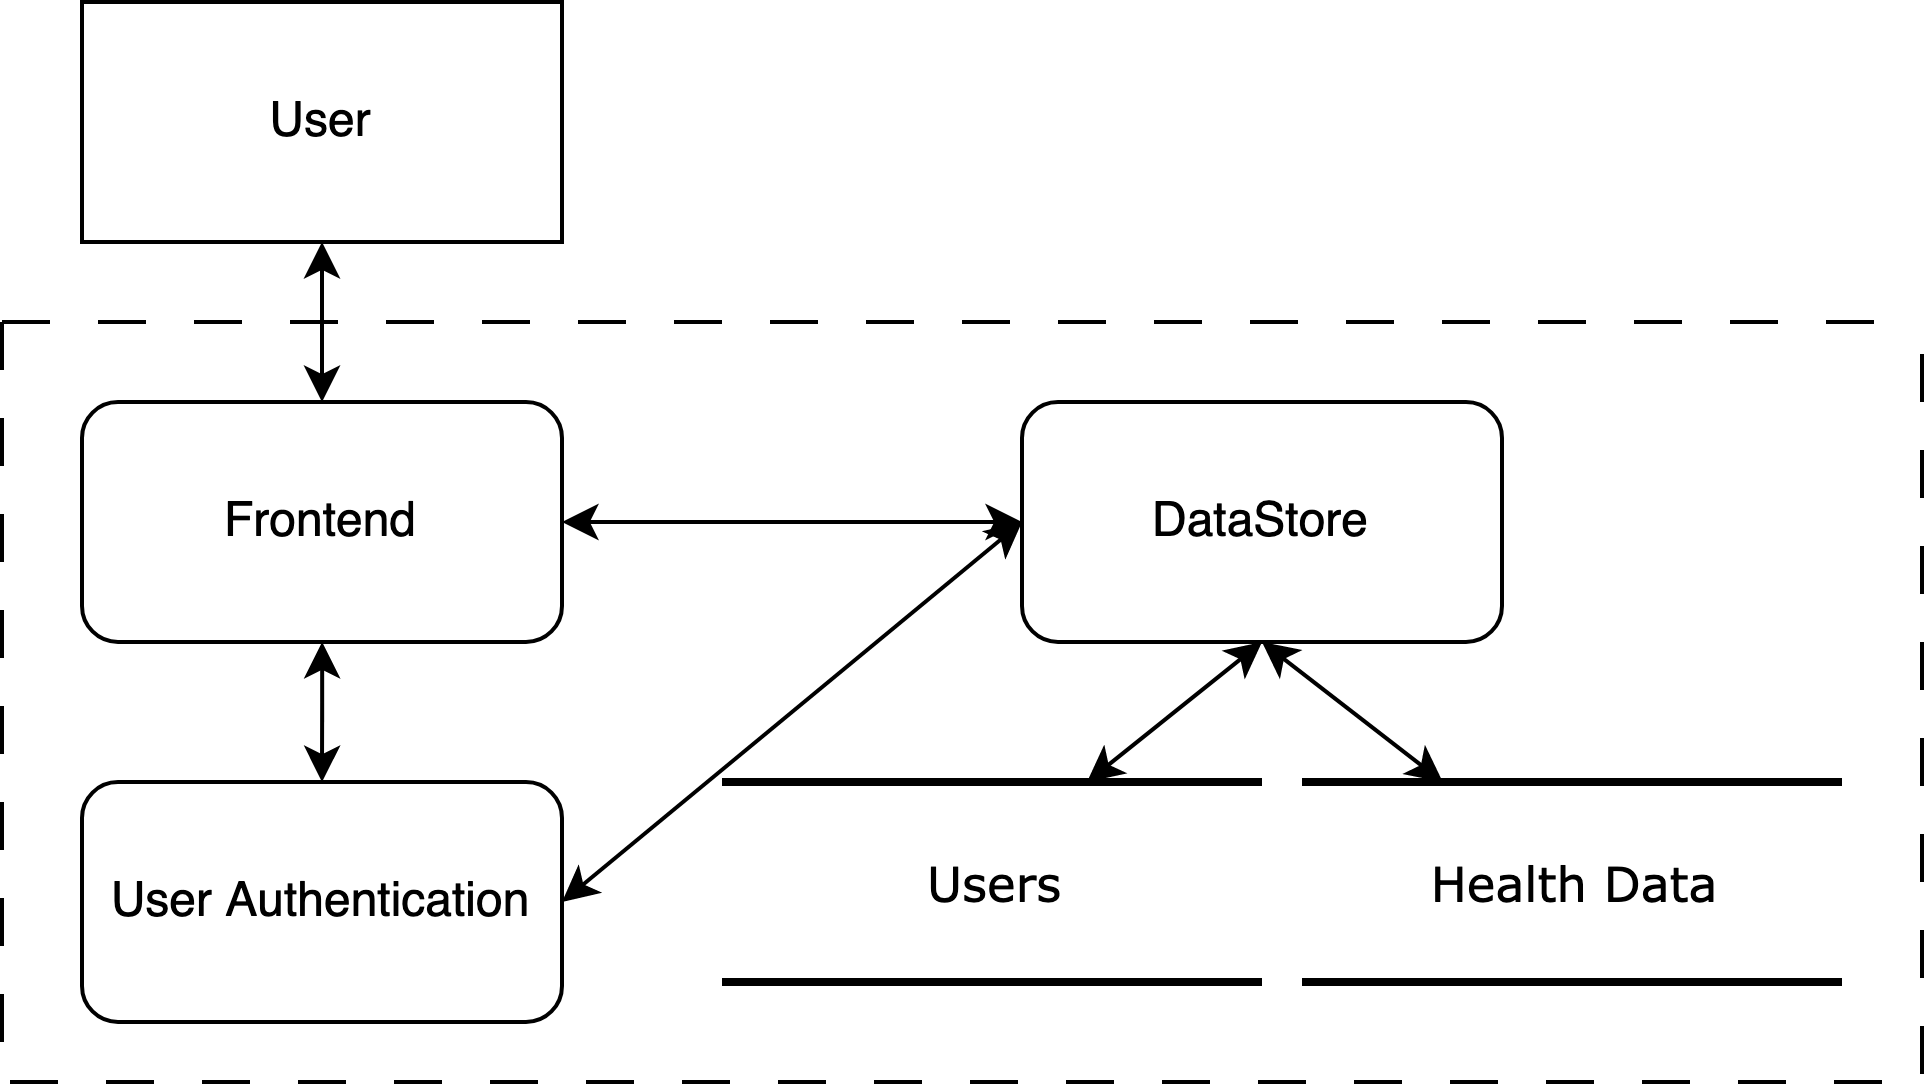
\includegraphics[width=\textwidth]{Diagrams/threat-modelling-1.png}
  \end{center}
\end{figure}
\subsection{Formulate STRIDE}
\textbf{Spoofing Identity}
\begin{itemize}
  \item Creation of fake user accounts
  \item Impersonation of existing users
\end{itemize}
\textbf{Tampering with Data}
\begin{itemize}
  \item Direct alterations of stored data
  \item Data corruption during transfer
\end{itemize}
\textbf{Repudiation}
\begin{itemize}
  \item Denying users access to data entry
  \item Denying users access to data deletion
\end{itemize}
\textbf{Information Disclosure}
\begin{itemize}
  \item Access to health data without being authorized
  \item Data leaks through debugging external debugging tools
\end{itemize}
\textbf{Denial of Service}
\begin{itemize}
  \item Intentionally crashing the app through malformed data
  \item Denying service through DDoS attacks
\end{itemize}
\textbf{Elevation of Privilege}
\begin{itemize}
  \item Access to admin features without proper authorization
  \item Exploiting vulnerabilities in the system to elevate user privileges
\end{itemize}

\subsection{Updated Fitness T racker App Flow Diagram}
\begin{figure}[H]
  \caption{Data Flow Diagram for the Fitness Tracker App}
  \vspace*{1em}
  \begin{center}
    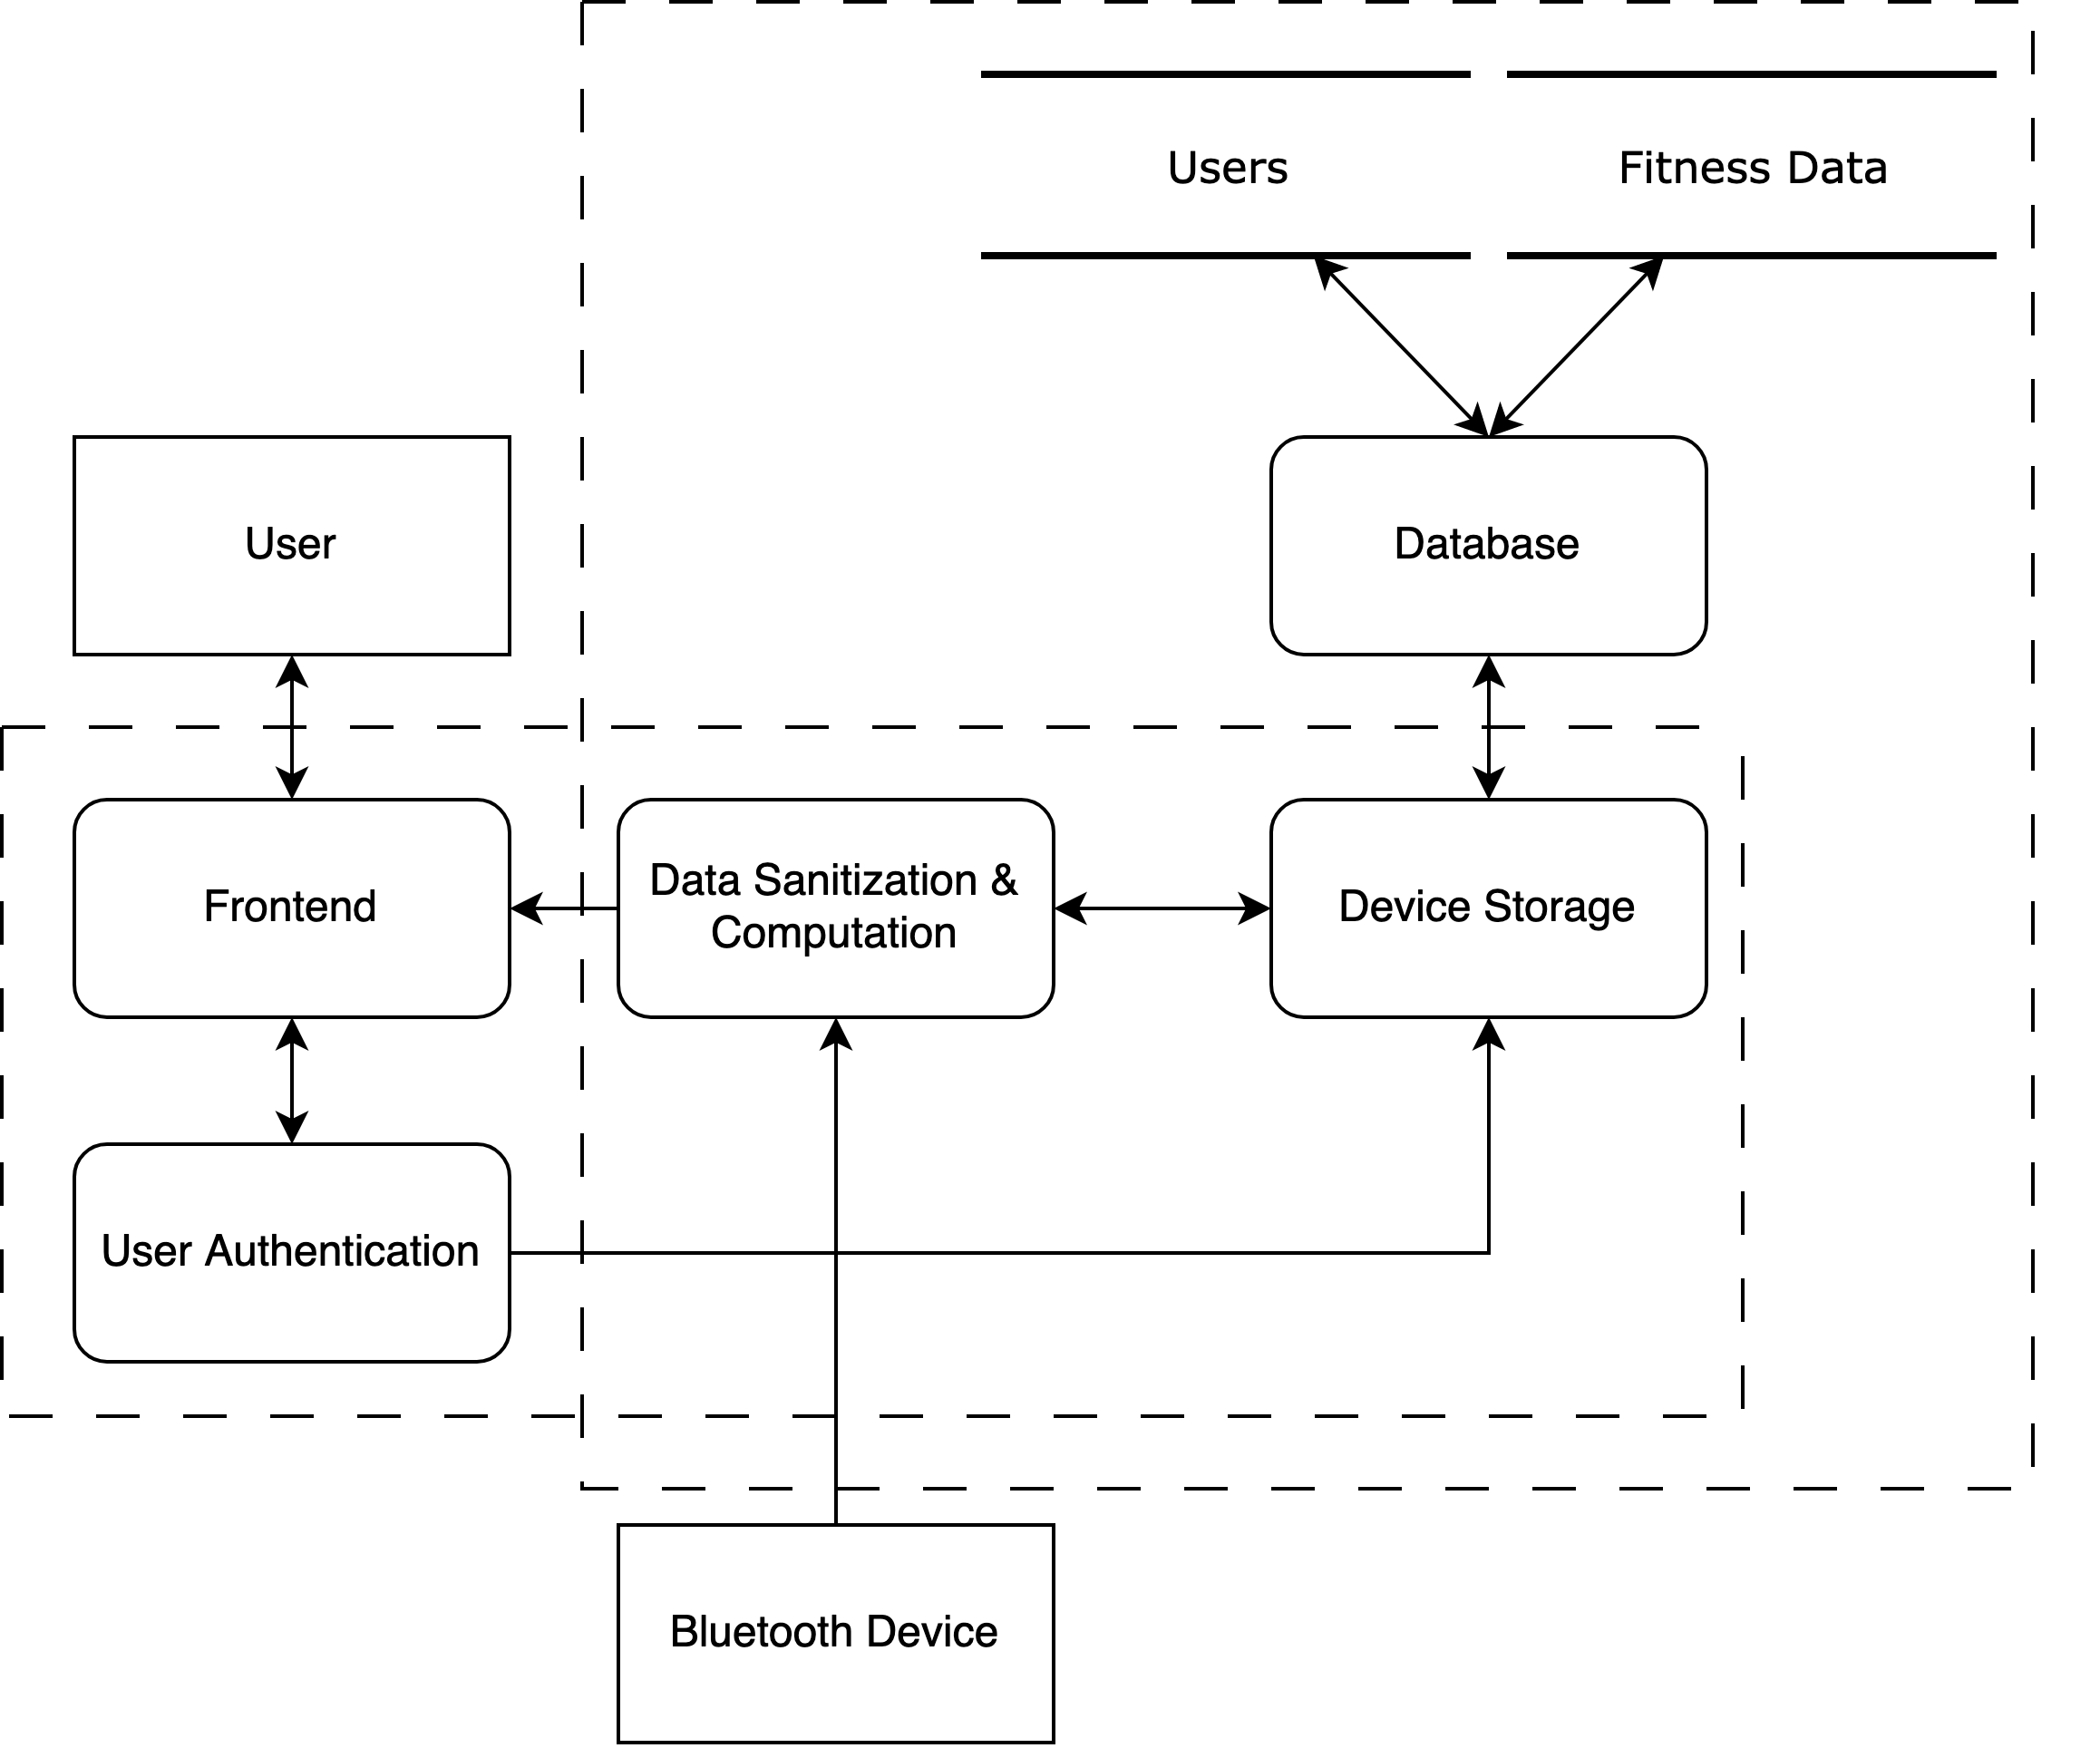
\includegraphics[width=\textwidth]{Diagrams/threat-modelling-2.png}
  \end{center}
\end{figure}
\subsection{Formulate STRIDE}
\textbf{Spoofing Identity}
\begin{itemize}
  \item Impersonation of a third-party devices such as a bluetooth device
  \item Impersonation of a fake cloud server that the app connects to
\end{itemize}
\textbf{Tampering with Data}
\begin{itemize}
  \item Direct alterations of stored data
  \item Data corruption during transfer
\end{itemize}
\textbf{Repudiation}
\begin{itemize}
  \item Denial of data transmission
  \item Denial of data processing
\end{itemize}
\textbf{Information Disclosure}
\begin{itemize}
  \item Unauthorized access to the stored fitness data on device as well as cloud
  \item Potential leaks via lacking security of third-party devices connecting to the app
\end{itemize}
\textbf{Denial of Service}
\begin{itemize}
  \item Sending large amounts of fitness tracking data, overloading the app server
  \item Cloud service could become unavailable, resulting in data sync between device and cloud not being possible
\end{itemize}
\textbf{Elevation of Privilege}
\begin{itemize}
  \item Unauthorized access to data on the cloud server without having necessary privileges
  \item Use exploits in the app to gain elevated access to cloud server
\end{itemize}

\end{document}